\section{Results}\label{sec:results}

Table~\ref{tab:confirmatory} summarises every confirmatory test. The subsections below
give the details and the exploratory analyses around them.

\begin{table}[p]
\centering
\footnotesize
\caption{All confirmatory tests. (a) Inference: estimates in percentage points with
95\% intervals (c1: 90\%, its prespecified decision rule). $p$ is the raw bootstrap
$p$-value (two-sided for differences, TOST for equivalence, one-sided for $R>0$);
``0/$10^4$'': no resample out of 10,000 crossed the boundary (95\% upper bound
$3\cdot10^{-4}$). $p_{\mathrm{H}}$: Holm within the family. (b) Best-of-32 accuracies (\%) under the prespecified grader; MV is
the verifier-independent majority vote.}\label{tab:confirmatory}
\resizebox{\linewidth}{!}{%
\begin{tabular}{lllrrl}
\multicolumn{6}{l}{(a) Inference}\\
\toprule
test & population ($n$) & contrast & estimate [CI] & $p$ & $p_{\mathrm{H}}$ \quad result \\
\midrule
c1 & main (1,200) & 8B ORM, W4 vs BF16 & $+0.33$ [$-0.58$, $+1.25$] & 0/$10^4$$^a$ & --$^a$ \quad equivalent \\
c2 & main (2,000) & 4B W4 packed vs 1.7B BF16 & $+2.25$ [$+1.05$, $+3.45$] & 0.0001 & 0.0005 \quad supported \\
c3 & -- & CH-GPTQ vs DPQ-adapted (not run) & -- & 1 & 1 \quad not tested \\
c4 & main MATH (1,200) & 4B+8B ORM, W4 vs BF16 & $-0.63$ [$-1.38$, $+0.08$] & 0.099 & 0.40$^b$ \quad not supported \\
c5 & main MATH (1,200) & loss growth, $N$=4$\to$32 & $-0.51$ [$-1.20$, $+0.16$] & 0.140 & 0.42$^b$ \quad not supported \\
\midrule
H6a & H6 (800) & 8B ORM, W4, $\pm3$ & $0.00$ [$-1.13$, $+1.13$] & 0/$10^4$ & 0/$10^4$ \quad equivalent \\
H6a & H6 (800) & PRM, W4, $\pm3$ & $+0.50$ [$-0.50$, $+1.50$] & 0/$10^4$ & 0/$10^4$ \quad equivalent \\
H6b & H6 (800) & 8B ORM, $R>0$ & $-1.88$ [$-3.19$, $-0.63$] & 0.998 & 0.998 \quad not supported \\
H6b & H6 (800) & PRM, $R>0$ & $+0.56$ [$-0.63$, $+1.69$] & 0.182 & 0.365 \quad not supported \\
\midrule
H7a & H7 (1,060) & 8B ORM, W4, $\pm3$ & $-0.28$ [$-1.42$, $+0.85$] & 0.0001 & 0.0002 \quad equivalent \\
H7a & H7 (1,060) & PRM, W4, $\pm3$ & $-0.57$ [$-1.32$, $+0.19$] & 0/$10^4$ & 0/$10^4$ \quad equivalent \\
H7b & H7 (1,060) & 8B ORM, $R>0$ & $+1.23$ [$-0.14$, $+2.59$] & 0.041 & 0.041 \quad supported \\
H7b & H7 (1,060) & PRM, $R>0$ & $+3.54$ [$+2.45$, $+4.72$] & 0/$10^4$ & 0/$10^4$ \quad supported \\
\bottomrule
\end{tabular}}

\smallskip
{\scriptsize
\begin{tabular}{llrrr}
\multicolumn{5}{l}{(b) Accuracies}\\
\toprule
test & verifier & BF16 & quantized & MV \\
\midrule
c1 & 8B ORM & 77.5 & 77.8 & 78.3 \\
c2 & 1.7B BF16 / 4B W4 packed & 71.8 & 74.1 & 72.1 \\
c4 & 4B and 8B ORM (mean) & 67.1 & 66.5 & 64.8 \\
H6 & 8B ORM / PRM & 72.8 / 76.6 & 72.8 / 77.1 & 76.5 \\
H7 & 8B ORM / PRM & 59.0 / 64.2 & 58.7 / 63.6 & 55.9 \\
\bottomrule
\end{tabular}}

\smallskip
\parbox{\linewidth}{\scriptsize $^a$\,c1 is judged by equivalence: its 90\% interval lies
inside $\pm3$\pp, and the TOST $p$-value is shown. The prespecified Holm family entered c1
with the two-sided $p$-value of its difference test (0.588, Holm 1.00), and the Holm values
of c4 and c5 shown here are computed with it. $^b$\,With the TOST $p$-value of c1 in the
family instead, the Holm-adjusted values of c4 and c5 would both be 0.30; no decision
changes.}
\end{table}

\subsection{Four-bit quantization preserves Best-of-32 accuracy}\label{sec:equivalence}

The prespecified contrast c1 uses the 8B ORM at GPTQ-W4 on the original 1,200-problem
manifest, where BF16 accuracy is 77.5\%. Quantization changes accuracy by $\Delta_{32} =
+0.33$\pp, with a 90\% interval of $[-0.58, +1.25]$. The interval lies inside the
prespecified $\pm3$\pp\ margin, and no bootstrap resample out of 10,000 fell beyond
either margin, so \textbf{equivalence is supported}. On this population a 3\pp\ loss
would have meant 13\% more errors. On the full 2,000 problems the same contrast is
$+0.15$\pp\ $[-0.65, +0.95]$ (95\% interval; Table~\ref{tab:main}).

Table~\ref{tab:main} gives the exploratory grid on the 2,000 problems. At 4 bits,
GPTQ-W4 and NF4 change $A_{32}$ by between $-1.1$ and $+0.6$\pp\ for the three ORMs and
the PRM, even though the selected candidate changes on 21--49\% of problems. The 4-bit
curves track BF16 at every budget $N\le32$ (Fig.~\ref{fig:curves}). Selection degrades
at 3 bits with this recipe. GPTQ-W3 costs 1.3--1.8\pp\ for the 4B ORM, the 8B ORM and
the PRM, and 13.2\pp\ for the 1.7B ORM, whose accuracy falls towards the
random-candidate rate. For the 4B and 8B ORMs the quantization method makes little
difference at 4 bits. Their $\Delta_{32}$ is $0.00$ and $+0.55$\pp\ with AWQ-W4, $+0.25$
and $+0.90$\pp\ with round-to-nearest (RTN-W4), and $+0.25$\pp\ with RTN-W8 on the 8B.
The 1.7B ORM is more sensitive to the method and loses $2.8$\pp\ $[-4.0, -1.7]$ with
RTN-W4, against $1.1$\pp\ with GPTQ-W4.

\begin{table}[!htb]
\centering
\small
\caption{Best-of-32 accuracy (\%) and change versus BF16 (pp, 95\% CI) in the main study
(2,000 problems, Qwen2.5-1.5B-Instruct candidates). Winner change is the share of
problems whose selected candidate differs from the BF16 one. Verifier-free baselines:
majority vote 72.1\%, oracle pass@32 86.9\%, random candidate 52.1\%.}\label{tab:main}
\begin{tabular}{llrrr}
\toprule
verifier & precision & $A_{32}$ & $\Delta_{32}$ [95\% CI] & winner change \\
\midrule
Skywork-1.7B & BF16 & 71.8 & -- & -- \\
 & NF4 & 70.7 & $-1.10$ [$-2.00$, $-0.25$] & 34\% \\
 & GPTQ-W4 & 70.7 & $-1.10$ [$-2.25$, $+0.05$] & 49\% \\
 & GPTQ-W3 & 58.7 & $-13.15$ [$-15.05$, $-11.25$] & 88\% \\
Skywork-4B & BF16 & 73.5 & -- & -- \\
 & NF4 & 72.7 & $-0.80$ [$-1.55$, $-0.10$] & 24\% \\
 & GPTQ-W4 & 74.1 & $+0.55$ [$-0.30$, $+1.40$] & 29\% \\
 & GPTQ-W3 & 71.8 & $-1.75$ [$-3.05$, $-0.45$] & 60\% \\
Skywork-8B & BF16 & 72.9 & -- & -- \\
 & NF4 & 72.9 & $-0.05$ [$-0.75$, $+0.65$] & 21\% \\
 & GPTQ-W4 & 73.1 & $+0.15$ [$-0.65$, $+0.95$] & 25\% \\
 & GPTQ-W3 & 71.3 & $-1.60$ [$-2.75$, $-0.45$] & 50\% \\
PRM-7B & BF16 & 76.6 & -- & -- \\
 & NF4 & 76.5 & $-0.05$ [$-0.65$, $+0.50$] & 25\% \\
 & GPTQ-W4 & 76.3 & $-0.30$ [$-1.05$, $+0.45$] & 33\% \\
 & GPTQ-W3 & 75.3 & $-1.30$ [$-2.30$, $-0.25$] & 54\% \\
\bottomrule
\end{tabular}
\end{table}

\begin{figure}[t]
\centering
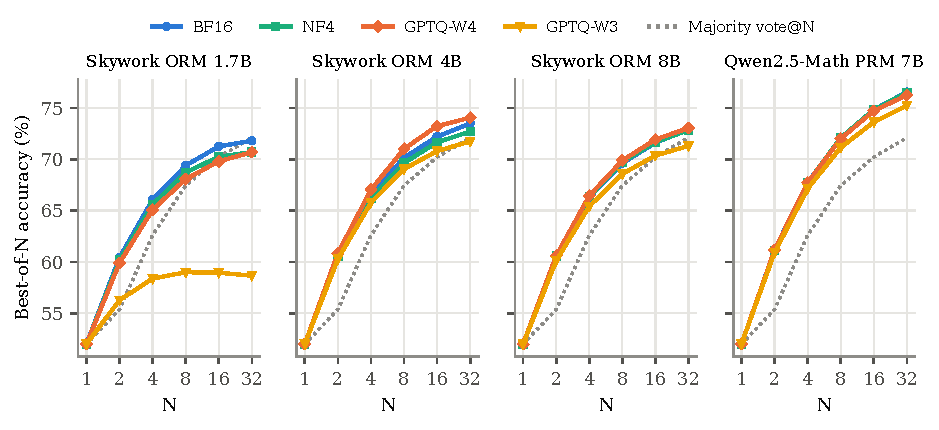
\includegraphics[width=\linewidth]{figures/curves.pdf}
\caption{Best-of-$N$ accuracy as a function of the number of candidates $N$, per
verifier and precision (main study, 2,000 problems; 200 random subsets per problem for
$N<32$). The dotted line is the verifier-free majority vote over the same $N$
candidates.}\label{fig:curves}
\end{figure}

\subsection{Under the 6~GiB verifier budget, the tested 4B 4-bit verifier is best}\label{sec:frontier}

Fig.~\ref{fig:frontier} shows accuracy against measured verifier memory for the tested
deployments. The plan states the ceiling as 6~GB, and we apply it to the GiB
measurements as 6~GiB. The selected configuration needs 4.92~GiB (5.3~GB) and fits under
either reading. The configuration selected on development data is the 4B ORM with packed
GPTQ-W4, and the best BF16 verifier that fits is the 1.7B ORM (4.02~GiB). The
prespecified contrast c2 is $+2.25$\pp\ $[+1.05, +3.45]$ ($p=0.0001$, Holm $p=0.0005$),
so the hypothesis is \textbf{supported}. The 1.7B BF16 verifier is 0.3\pp\ below
majority vote, which needs no verifier, and the 4B GPTQ-W4 verifier is 2.0\pp\ above
it. The comparison applies to the tested checkpoints, the fixed scoring workload and
verifier memory only. In this family accuracy does not grow with size (the 4B BF16
model beats the 8B), so the result describes these deployments and does not imply that
larger verifiers are generally better.

Part of the advantage comes from answer format, and its size depends on the selection
policy. Three secondary analyses, each applied identically to both arms, give a
consistent but smaller effect. With the lenient grader, c2 is $+1.55$\pp\ $[+0.45,
+2.65]$. Restricting Best-of-32 to candidates with an extractable answer gives 75.4\%
versus 74.0\%, a difference of $+1.40$\pp\ $[+0.35, +2.45]$, and a reward-weighted vote
gives 75.5\% versus 74.0\%, $+1.50$\pp\ $[+0.45, +2.55]$. Finally, one of the authors
graded every distinct Best-of-32 winner without an extractable answer in either arm (94
responses), together with 30 random winners with one, without knowing the arm, the
verifier or the grader's verdict (\ref{app:audit}). Replacing the strict grader by these
labels gives $+1.40$\pp\ $[+0.30, +2.50]$ (75.5\% versus 74.1\%, nominal $p=0.011$).
This interval treats the single rater's labels as error-free. None of the three analyses
belongs to the prespecified family. Together they suggest that the deployment advantage
under format-robust grading or selection is about 1.4--1.5\pp, and that the
strict-grader estimate is an upper value. The strict-grader contrast also stays
positive with revised GSM8K labels ($+2.37$\pp) and after excluding truncated
candidates ($+2.20$\pp).

\begin{table}[!htb]
\centering
\small
\caption{Peak verifier memory and scoring throughput on an RTX 4090 (exploratory
re-measurement with a fixed workload of 64 sequences of 900 tokens and no generator
resident). Peak allocated memory is recorded over one pass. Throughput is averaged over
three timed forward passes after one warm-up pass, with GPU synchronisation. The
re-measured peaks match the prespecified measurement used for c2 to within
0.001~GiB. The PRM has no packed GPTQ deployment (Section~\ref{sec:precisions}).}\label{tab:systems}
\begin{tabular}{lrrrrrr}
\toprule
 & \multicolumn{2}{c}{BF16} & \multicolumn{2}{c}{NF4 (\texttt{bitsandbytes})} & \multicolumn{2}{c}{GPTQ-W4 (packed)} \\
verifier & GiB & seq/s & GiB & seq/s & GiB & seq/s \\
\midrule
Skywork-1.7B & 4.02 & 38.0 & 2.13 & 37.6 & 2.07 & 36.7 \\
Skywork-4B & 9.95 & 16.5 & 5.08 & 16.3 & 4.92 & 16.0 \\
Skywork-8B & 16.97 & 9.8 & 7.67 & 9.7 & 7.37 & 9.7 \\
PRM-7B & 16.72 & 11.4 & 7.98 & 11.2 & -- & -- \\
\bottomrule
\end{tabular}
\end{table}

The re-measurement (Table~\ref{tab:systems}) adds the PRM, which needs 16.72~GiB in
BF16 and 7.98~GiB with deployed NF4; the deployed NF4 scores are identical to the
simulated ones. With the PRM included, the best tested deployment under an 8~GiB budget
is the NF4 PRM (76.5\%), ahead of every ORM deployment, while the 6~GiB comparison of c2
is unchanged. Scoring throughput with 4-bit weights was 0.8--3.4\% lower than with BF16.
The workload is a large prefill batch of 57,600 tokens per pass, in which the smaller
weights do not speed up computation and dequantization adds a small cost. We did not
measure small batches, end-to-end latency or a generator resident on the same GPU. For
scale, the generators' BF16 weights alone take about 2.9~GiB (Qwen2.5-1.5B), 6.0~GiB
(Llama-3.2-3B) and 14.2~GiB (Qwen2.5-Math-7B), computed from their parameter counts and
excluding the key--value cache.

\begin{figure}[t]
\centering
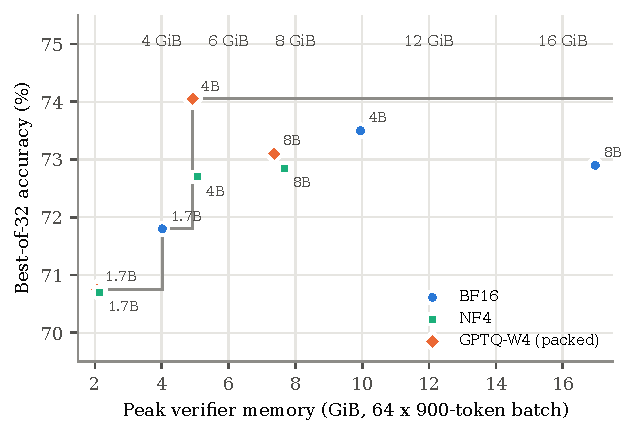
\includegraphics[width=0.75\linewidth]{figures/frontier.pdf}
\caption{Accuracy against measured verifier memory for the tested Skywork ORM and PRM
deployments (Best-of-32, main study, 2,000 problems; PRM memory from the exploratory
re-measurement). Memory is the peak allocation while scoring a fixed workload of 64
sequences of 900 tokens on an RTX 4090 with no generator. GPTQ-W4 uses packed 4-bit
kernels and NF4 uses \texttt{bitsandbytes}. Vertical lines mark the prespecified
ceilings, and the dashed one is the 6~GiB ceiling of c2. The step line is the envelope of
the tested neural-verifier deployments within each budget. Majority vote (dotted) needs
no verifier memory and beats every tested verifier deployment below
4.9~GiB.}\label{fig:frontier}
\end{figure}

\subsection{Selected candidates change often, selected answers much less often}\label{sec:mechanism}

Table~\ref{tab:transitions} breaks the 4-bit and 3-bit changes down into answer
transitions. With GPTQ-W4 or NF4 the selected candidate changes on 21--49\% of
main-study problems, but the selected canonical answer changes on only 4.8--13.2\%, and
72--79\% of the candidate changes keep the same final answer. Harm (a correct BF16
selection becomes wrong) and benefit (the reverse) each affect 0.9--4.1\% of problems
and largely cancel. At 3 bits the answer-change rate (14.2--38.9\%) and harm both grow,
and harm exceeds benefit. H6 and H7 show the same pattern. These measurements are
consistent with answer redundancy in the pools. Candidates that share the selected
answer are interchangeable for accuracy, so most score perturbations move the selection
within the same answer cluster.

\begin{table}[!htb]
\centering
\small
\caption{Answer transitions at $N=32$ relative to BF16 (\% of problems). Cand.: selected
candidate changes; answer: selected canonical answer changes; same: share of candidate
changes that keep the answer; harm: correct $\to$ wrong; benefit: wrong $\to$ correct;
$\Delta_{32}$ = benefit $-$ harm (pp). A switch between two winners without an
extractable answer counts as an answer change. Some such switches are between prose
answers a human would judge equal, so the answer column is an upper value, most of all
for the ORMs that prefer prose answers.}\label{tab:transitions}
\resizebox{\linewidth}{!}{%
\begin{tabular}{lllrrrrrr}
\toprule
study & verifier & condition & cand. & answer & same & harm & benefit & $\Delta_{32}$ \\
\midrule
main & ORM 1.7B & GPTQ-W4 & 48.9 & 13.2 & 73 & 4.1 & 3.0 & $-1.10$ \\
 & & GPTQ-W3 & 87.6 & 38.9 & 56 & 17.7 & 4.5 & $-13.15$ \\
 & ORM 4B & GPTQ-W4 & 29.2 & 8.1 & 72 & 1.7 & 2.3 & $+0.55$ \\
 & & GPTQ-W3 & 59.7 & 17.7 & 70 & 5.2 & 3.5 & $-1.75$ \\
 & ORM 8B & BF16-null & 6.9 & 1.0 & 86 & 0.3 & 0.2 & $-0.10$ \\
 & & NF4 & 21.2 & 4.8 & 78 & 1.3 & 1.2 & $-0.05$ \\
 & & GPTQ-W4 & 25.1 & 6.2 & 76 & 1.5 & 1.7 & $+0.15$ \\
 & & GPTQ-W3 & 50.5 & 14.2 & 72 & 4.3 & 2.7 & $-1.60$ \\
 & PRM & NF4 & 25.2 & 5.7 & 78 & 0.9 & 0.9 & $-0.05$ \\
 & & GPTQ-W4 & 33.0 & 7.1 & 79 & 1.6 & 1.3 & $-0.30$ \\
 & & GPTQ-W3 & 54.0 & 14.3 & 74 & 3.4 & 2.1 & $-1.30$ \\
\midrule
H6 & ORM 8B & GPTQ-W4 & 31.4 & 6.9 & 78 & 1.3 & 1.3 & $0.00$ \\
 & PRM & GPTQ-W4 & 34.4 & 5.8 & 83 & 0.8 & 1.3 & $+0.50$ \\
H7 & ORM 8B & GPTQ-W4 & 26.9 & 8.8 & 67 & 2.1 & 1.8 & $-0.28$ \\
 & PRM & GPTQ-W4 & 30.1 & 8.7 & 71 & 1.0 & 0.5 & $-0.57$ \\
 & ORM 8B & GPTQ-W3 & 51.7 & 20.6 & 60 & 5.8 & 2.3 & $-3.49$ \\
 & PRM & GPTQ-W3 & 55.9 & 20.4 & 64 & 3.8 & 1.2 & $-2.55$ \\
\bottomrule
\end{tabular}}
\end{table}

\begin{figure}[t]
\centering
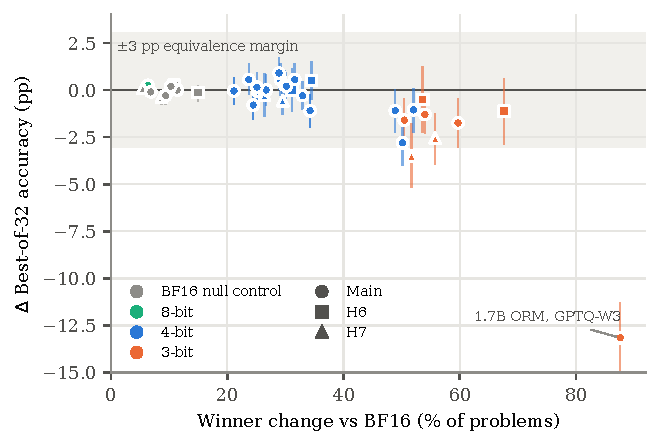
\includegraphics[width=0.75\linewidth]{figures/mechanism.pdf}
\caption{Winner change versus accuracy change at $N=32$ for every quantized condition
and control in the main study (circles) and the two follow-up studies (H6 squares, H7
triangles), with 95\% bootstrap intervals. The exploratory revision experiments
(Llama-based ORMs, in-domain calibration) are not shown. Four-bit conditions change the
selected candidate on 21--52\% of problems, with point estimates inside the $\pm3$\pp\
band. Three-bit conditions change about half or more of the winners and lose
accuracy.}\label{fig:mechanism}
\end{figure}

\subsection{No confirmatory evidence for the MATH-loss and budget-growth contrasts}\label{sec:c4c5}

Development data had suggested that quantization damage concentrates on MATH and grows
with $N$. On the 1,200 evaluation MATH problems, c4 (the MATH $\Delta_{32}$ of the 4B
and 8B ORMs at GPTQ-W4, averaged within problem) is $-0.63$\pp\ $[-1.38, +0.08]$ with
Holm $p=0.40$. c5, the change of that loss from $N=4$ to $N=32$, is $-0.51$\pp\
$[-1.20, +0.16]$ with Holm $p=0.42$. Neither hypothesis is supported. The results are
inconclusive and do not show that the effect is zero, although the intervals rule out
MATH losses larger than about 1.4\pp. c4 measures the loss within MATH and does not test
an interaction with difficulty. The development signal came from 200 problems and did
not replicate.

\subsection{A stronger generator on hard problems (H6)}\label{sec:h6}

H6 tested whether the result holds with a stronger generator on harder, previously
unused problems. Qwen2.5-Math-7B-Instruct \cite{yang2024qwen25math} generated 32
candidates of up to 2,048 tokens for 800 MATH Level-5 test problems, which the 8B ORM and
the PRM scored in BF16 and GPTQ-W4. The family of four tests asked for equivalence at
$\pm3$\pp\ (H6a) and for retention of at least half of the BF16 verifier's advantage
over majority vote (H6b). Let $G = A_{\mathrm{BF16}} - A_{\mathrm{MV}}$ be the BF16
advantage and $\Delta$ the quantization effect. H6b then tests
\[
R \;=\; \tfrac12 G + \Delta \;=\; (A_{\mathrm{Q}} - A_{\mathrm{MV}}) - \tfrac12 G \;>\; 0,
\]
that is, whether the quantized verifier's advantage exceeds half of the BF16 advantage.
$R$ is computed per problem as $R_i = C_{\mathrm{Q},i} - \tfrac12(C_{\mathrm{BF16},i} +
C_{\mathrm{MV},i})$ and bootstrapped as a mean. $R>0$ implies retained value only when
$G>0$, so the plans interpret H6b and H7b only for verifiers with a positive BF16
advantage, which we check descriptively with 97.5\% intervals.

Equivalence is supported for both verifiers, with $\Delta_{32} = 0.00$\pp\ $[-1.13,
+1.13]$ for the ORM and $+0.50$\pp\ $[-0.50, +1.50]$ for the PRM, although the selected
candidate changes on 31\% and 34\% of problems. With this generator, however, neither
verifier showed a clear advantage over majority vote (76.5\%). The PRM tied it ($G =
+0.13$\pp\ $[-1.88, +2.13]$) and the ORM fell below it ($G = -3.75$\pp\ $[-6.25,
-1.25]$). H6 therefore did not establish a positive BF16 advantage to retain, which
limits what its retention tests can show (ORM $R = -1.88$\pp, PRM $+0.56$\pp; neither
supported). These conclusions hold under the lenient grader and without truncated
candidates. Truncation is more common here than in the main study: 19\% of candidates
reached the length limit, all 32 candidates were truncated on 7 of the 800 problems, and
at least three quarters were truncated on 58.

\subsection{Value retention where the verifier adds value (H7)}\label{sec:h7}

H7 is a prospective follow-up targeted at a regime chosen from earlier exploratory
data, namely the main generator on hard problems, where the main-study PRM and 8B ORM had
beaten majority vote. It uses all 1,060 MATH Level-4 and Level-5 test problems not used
anywhere else in this work, the prespecified generation settings, and the same
verifiers, conditions, tests and analysis code as H6. Because the regime was chosen with
knowledge of earlier results, H7 estimates the effect of quantization in that regime. It
does not estimate the typical value of a verifier across deployments.

On the new problems both verifiers beat majority vote in BF16, the PRM by $+8.2$\pp\
(97.5\% interval $[+5.9, +10.7]$) and the 8B ORM by $+3.0$\pp\ $[+0.4, +5.8]$. All four
prespecified hypotheses are supported (Holm over four). Accuracy is equivalent at
$\pm3$\pp, with $\Delta_{32} = -0.28$\pp\ $[-1.42, +0.85]$ for the ORM and $-0.57$\pp\
$[-1.32, +0.19]$ for the PRM. Both quantized verifiers keep more than half of their BF16
advantage. The evidence is strong for the PRM ($R = +3.54$\pp\ $[+2.45, +4.72]$, Holm
$p \le 0.0003$) and narrow for the ORM ($R = +1.23$\pp\ $[-0.14, +2.59]$, one-sided Holm
$p = 0.041$), in line with the ORM's lower planned power. Descriptively, the PRM retains
93\% of its advantage (95\% interval 84--102\%) and the ORM 91\% (44--149\%). The ORM's
interval is wide because its BF16 advantage, the denominator of the ratio, is small. The
retention conclusions keep their sign under the lenient grader and without truncated
candidates, which the plan required before describing value as preserved. In an
exploratory comparison, three bits is not safe in this regime: GPTQ-W3 costs $3.5$\pp\
for the ORM and $2.6$\pp\ for the PRM and removes the ORM's advantage. Level-wise
estimates and all sensitivity analyses are in the repository, and
Fig.~\ref{fig:retention} summarises the advantage over majority vote before and after
quantization across regimes.

\begin{figure}[t]
\centering
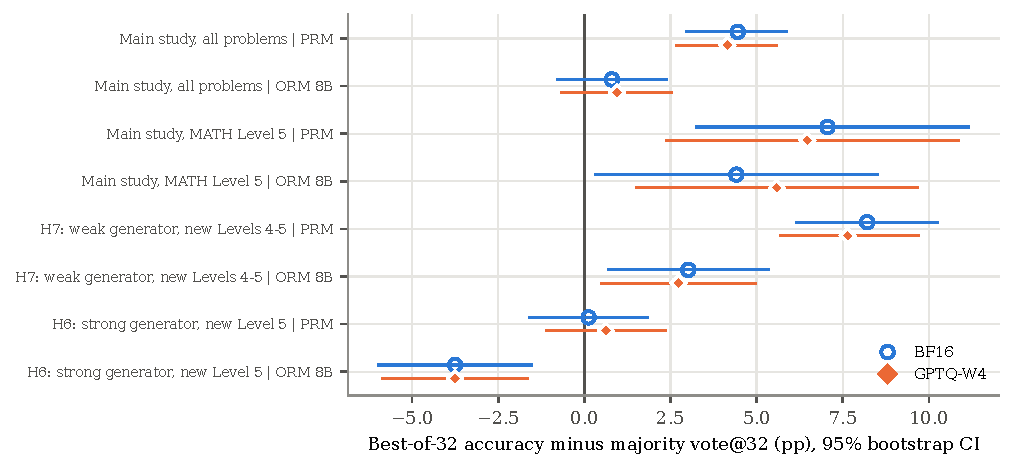
\includegraphics[width=\linewidth]{figures/retention.pdf}
\caption{Verifier advantage over majority vote (Best-of-32 accuracy minus majority
vote@32, pp, with 95\% bootstrap intervals) in BF16 (open circles) and with GPTQ-W4
(diamonds), for the 8B ORM and the PRM. Main-study rows are exploratory subsets; H6 and
H7 are separately planned studies on new problems.}\label{fig:retention}
\end{figure}

\subsection{Robustness and controls}\label{sec:robustness}

\paragraph{Other reward-model families} As an exploratory extension, we scored the
previously analysed main and H7 pools with two further ORMs on a Llama~3.1 backbone
(Table~\ref{tab:otherrm}). The 4-bit result holds within the $\pm3$\pp\ margin, with
somewhat larger losses than for the Skywork-Qwen models. GPTQ-W4 changes the accuracy of
Llama-3.1-Tulu-3-8B-RM by $-0.60$\pp\ on the main problems and $-0.75$\pp\ on H7, and
that of Skywork-Reward-V2-Llama-3.1-8B by $-1.45$\pp\ and $-1.23$\pp. All four 90\%
intervals lie inside $\pm3$\pp, but the Skywork-Llama loss on the main problems is
distinguishable from zero. Both models changed the selected candidate (44--53\%) and the
selected answer (11--25\%) more often than the Skywork-Qwen ORMs. Neither showed a clear
advantage $G$ over majority vote in BF16, so value retention cannot be interpreted for
them. With generic calibration at 3 bits, both Llama-based models break down. GPTQ-W3
costs Tulu-3 $12.6$\pp\ and Skywork-Llama $26.4$\pp, which puts the latter below the
random-candidate rate, against $1.6$\pp\ for the Qwen-based 8B ORM. With generic
calibration the 3-bit behaviour is therefore strongly model-dependent; for Tulu-3,
in-domain calibration recovers most of the loss (next paragraph).

\begin{table}[!htb]
\centering
\small
\caption{Exploratory results for the two Llama-3.1-based ORMs (Best-of-32). $A$: BF16
accuracy (\%); $\Delta$: change with GPTQ-W4 (pp) with 95\% and 90\% intervals; $G$:
BF16 advantage over majority vote (pp, 95\% interval; majority vote 72.1\% on the main
problems and 55.9\% on H7); cand./answer: share of problems whose selected candidate or
answer changes (\%). GPTQ-W3 with generic calibration on the main problems: Tulu-3
$-12.60$ $[-14.40, -10.75]$, answer change 35\%; Skywork-Llama $-26.35$ $[-28.70,
-24.05]$, answer change 59\%.}\label{tab:otherrm}
\resizebox{\linewidth}{!}{%
\begin{tabular}{llrrrrrr}
\toprule
ORM & population & $A$ & $\Delta$ [95\% CI] & 90\% CI & $G$ [95\% CI] & cand. & answer \\
\midrule
Tulu-3-8B-RM & main (2,000) & 72.5 & $-0.60$ [$-1.65$, $+0.45$] & [$-1.45$, $+0.30$] & $+0.35$ [$-1.20$, $+1.85$] & 44.6 & 11.5 \\
 & H7 (1,060) & 55.0 & $-0.75$ [$-2.45$, $+0.85$] & [$-2.17$, $+0.57$] & $-0.94$ [$-3.11$, $+1.23$] & 43.6 & 18.3 \\
Skywork-Llama-8B & main (2,000) & 68.8 & $-1.45$ [$-2.75$, $-0.15$] & [$-2.55$, $-0.35$] & $-3.35$ [$-5.05$, $-1.65$] & 51.7 & 18.3 \\
 & H7 (1,060) & 53.8 & $-1.23$ [$-3.11$, $+0.66$] & [$-2.74$, $+0.38$] & $-2.17$ [$-4.62$, $+0.28$] & 53.2 & 24.7 \\
\bottomrule
\end{tabular}}
\end{table}

\paragraph{Task-matched calibration at 3 bits} Much of the 3-bit loss depends on the
calibration data (exploratory; Table~\ref{tab:calib}). The prespecified recipe uses 128
WikiText chunks of exactly 512 tokens. The in-domain alternative uses 128 complete
candidate responses sampled from the generator's development pools, in the verifier's
input format and of variable length (about 490--540 tokens on average, depending on the
tokenizer). The calibration problems are development problems, disjoint from the
evaluation set. With the in-domain recipe, the loss of the 1.7B ORM falls from
$13.15$ to $3.75$\pp, and that of Tulu-3, a Llama-based ORM, from $12.60$ to $2.80$\pp.
The recoveries are $+9.40$\pp\ and $+9.80$\pp. For the verifiers that lost little with
generic calibration the change is smaller: $+1.55$\pp\ for the 8B ORM and $+0.70$\pp\
$[-0.35, +1.75]$ for the PRM, whose interval includes zero. A length control rules out
sequence length as the explanation. Calibrating the 1.7B ORM on WikiText cut to exactly
the token lengths of its in-domain set gives $\Delta_{32} = -16.75$\pp, no better than
the generic recipe and $13.00$\pp\ $[11.00, 14.95]$ worse than in-domain calibration.
The recovery therefore comes from the content of the calibration text, its domain or
its format, which this design does not separate. For the tested verifiers, the 3-bit
boundary we observe depends on the calibration recipe as well as on the bit width.
Skywork-Llama was not re-quantized with the in-domain recipe.

\begin{table}[!htb]
\centering
\small
\caption{GPTQ-W3 with generic and in-domain calibration (exploratory, main study, 2,000
problems, Best-of-32). $\Delta_{32}$ versus BF16 and the paired difference, in pp with
95\% intervals. Length control for the 1.7B ORM: WikiText cut to the token lengths of
its in-domain set, $\Delta_{32} = -16.75$ $[-18.75, -14.80]$.}\label{tab:calib}
\resizebox{\linewidth}{!}{%
\begin{tabular}{lrrrr}
\toprule
verifier & BF16 $A_{32}$ (\%) & generic $\Delta_{32}$ & in-domain $\Delta_{32}$ & in-domain $-$ generic \\
\midrule
Skywork-1.7B & 71.8 & $-13.15$ [$-15.05$, $-11.25$] & $-3.75$ [$-5.25$, $-2.30$] & $+9.40$ [$+7.55$, $+11.30$] \\
Skywork-8B & 72.9 & $-1.60$ [$-2.75$, $-0.45$] & $-0.05$ [$-1.00$, $+0.90$] & $+1.55$ [$+0.40$, $+2.75$] \\
PRM-7B & 76.6 & $-1.30$ [$-2.30$, $-0.25$] & $-0.60$ [$-1.45$, $+0.25$] & $+0.70$ [$-0.35$, $+1.75$] \\
Tulu-3-8B-RM & 72.5 & $-12.60$ [$-14.40$, $-10.75$] & $-2.80$ [$-4.00$, $-1.65$] & $+9.80$ [$+7.95$, $+11.60$] \\
\bottomrule
\end{tabular}}
\end{table}

\paragraph{Selection rules} The 4-bit result does not depend on the selection rule
(exploratory, main study, $N=32$). In the reward-weighted answer vote each candidate
with an extractable answer adds $\mathrm{softmax}(s/T)$ to its answer cluster, where $s$
is the verifier score and $T$ is fitted on development data in BF16 and kept fixed
across precisions ($T=0.3$ for the 8B ORM and $0.1$ for the other verifiers). Under
reward-weighted voting, BF16 accuracy and its change with GPTQ-W4 are 73.95\%
($-1.00$\pp) for the 1.7B ORM, 76.00\% ($-0.60$\pp) for the 4B ORM, 76.20\%
($+0.30$\pp) for the 8B ORM and 79.50\% ($+0.25$\pp) for the PRM. Restricting
Best-of-32 to candidates with an extractable answer gives 73.95\% ($-1.10$\pp), 75.95\%
($-0.55$\pp), 76.10\% ($0.00$\pp) and 79.75\% ($-0.45$\pp) for the same four verifiers,
and last-step aggregation for the PRM gives 79.35\% ($-0.25$\pp). GPTQ-W3 loses
0.7--11\pp\ under every rule. Restricting selection to extractable answers raises the
BF16 ORMs' accuracy by 2.2--3.2\pp\ (for the 8B ORM, from 72.9\% to 76.1\%), which shows
how much the strict grader penalises their preference for prose answers. Under both
rules the c2 contrast stays positive ($+1.40$ and $+1.50$\pp;
Section~\ref{sec:frontier}).

\paragraph{Answer format} Under the strict grader several quantized conditions appeared
to \emph{improve} GSM8K accuracy, for example by $+3.0$\pp\ for the 4B ORM at GPTQ-W4
and by $+8.0$\pp\ on the Llama pools. The format/content decomposition
(Section~\ref{sec:grading}) shows that these gains come from answer format. Quantization
weakens the Skywork ORMs' preference for prose answers without a boxed final answer. For
the 4B ORM at GPTQ-W4 the format term is $+3.0$\pp\ and the content term $0.0$\pp, and
the difference under the lenient grader is $+0.4$\pp. On MATH the changes come from
answer content under both graders. We therefore claim no accuracy gain from
quantization.

\paragraph{Packed versus simulated quantization} Packed GPTQ-W4, which runs FP16 Marlin
kernels, and simulated GPTQ-W4, which runs in BF16, select the same final answer on
98.8--99.2\% of problems and the same candidate on 84.7--88.8\%. Their candidate-level
disagreement (11.3--15.4\%) is somewhat larger than the bf16-null floor (6.9--11\%), and
their answer-level disagreement (0.8--1.2\%) is of the same size as the null control's
(1.0\% for the 8B ORM). Correctness flips are rare and symmetric (0.35--0.55\% of
problems). Packed GPTQ-W4 changes accuracy versus BF16 by $-1.05$, $+0.55$ and
$+0.20$\pp\ for the 1.7B, 4B and 8B ORMs, against $-1.10$, $+0.55$ and $+0.15$\pp\ for
simulated quantization. c2 uses the packed scores.

\paragraph{Second generator} On 300 problems with Llama-3.2-3B-Instruct candidates
(exploratory), GPTQ-W4 changes the PRM's Best-of-32 accuracy by $+0.33$\pp\ $[-3.00,
+4.00]$ and NF4 by $-0.67$\pp. For the 4B ORM the strict grader shows $+8.0$\pp, which
shrinks to $+2.0$\pp\ $[0.0, +4.3]$ under the lenient grader, again a format effect.
With this generator, majority vote (76.3\%) beats both verifiers in BF16 (ORM 63.7\%,
PRM 70.7\%).

\paragraph{Labels and truncation} With GSM8K-Platinum labels the c1 estimate is
$+0.44$\pp. c4 and c5 involve MATH only and do not change. With truncated candidates
removed before selection, the estimates are $+0.33$\pp\ for c1, $-0.67$\pp\ for c4 and
$-0.52$\pp\ for c5. None of these sensitivity estimates reverses the direction of a
prespecified conclusion. Both GSM8K problems whose labels the human audit had flagged as
questionable are among those that GSM8K-Platinum removes.
